\subsection{KAGE} \label{background:kage}
KAGE \cite{kage} is an alignment-free genotyping tool for SNPs and short indels.
Unlike alignment-based genotyping tools, KAGE uses an alignment-free method that does not align sequenced reads to a reference genome.
Instead, KAGE counts the occurrences of a predefined set of \textit{k}mers in the input reads to then directly compute the likelihood of every possible genotype ($0/0$, $0/1$ or $1/1$) being present for each variant in an input set of known variants.
These probabilities are based on the observed \textit{k}mer counts in the reads and the expected \textit{k}mer counts for an individual who carries the particular genotype.
The expected \textit{k}mer counts for each genotype are estimated beforehand based on large catalogues of genotype data accumulated over many years of research from projects such as the 1000 Genomes Project \cite{1000_genomes_project}.
Indices of estimated expected \textit{k}mer counts are created once and then re-used for many consecutive genotyping runs.
KAGE recently showed (2022) that its accuracy was on par with the best existing alignment-free genotyping tools while being an order of magnitude faster \cite{kage}.

KAGE is implemented in Python and relies extensively on the NumPy library for performance.
Its genotyping pipeline is split into two distinct programs: \textit{kmer\_mapper}, solving the \textit{partial} \textit{k}mer counting problem of counting \textit{k}mer frequencies for a predefined set of \textit{k}mers in the input reads, and \textit{kage}, which finally computes the genotype-probabilities based on the \textit{k}mer counts provided by \textit{kmer\_mapper}.
We will use KAGE to refer to the full KAGE genotyping pipeline, and \textit{kage} to refer to the piece of software the performs the genotype-probability computations, which is one component of the total pipeline.

\begin{figure}[H]
\begin{center}
\scalebox{1}{
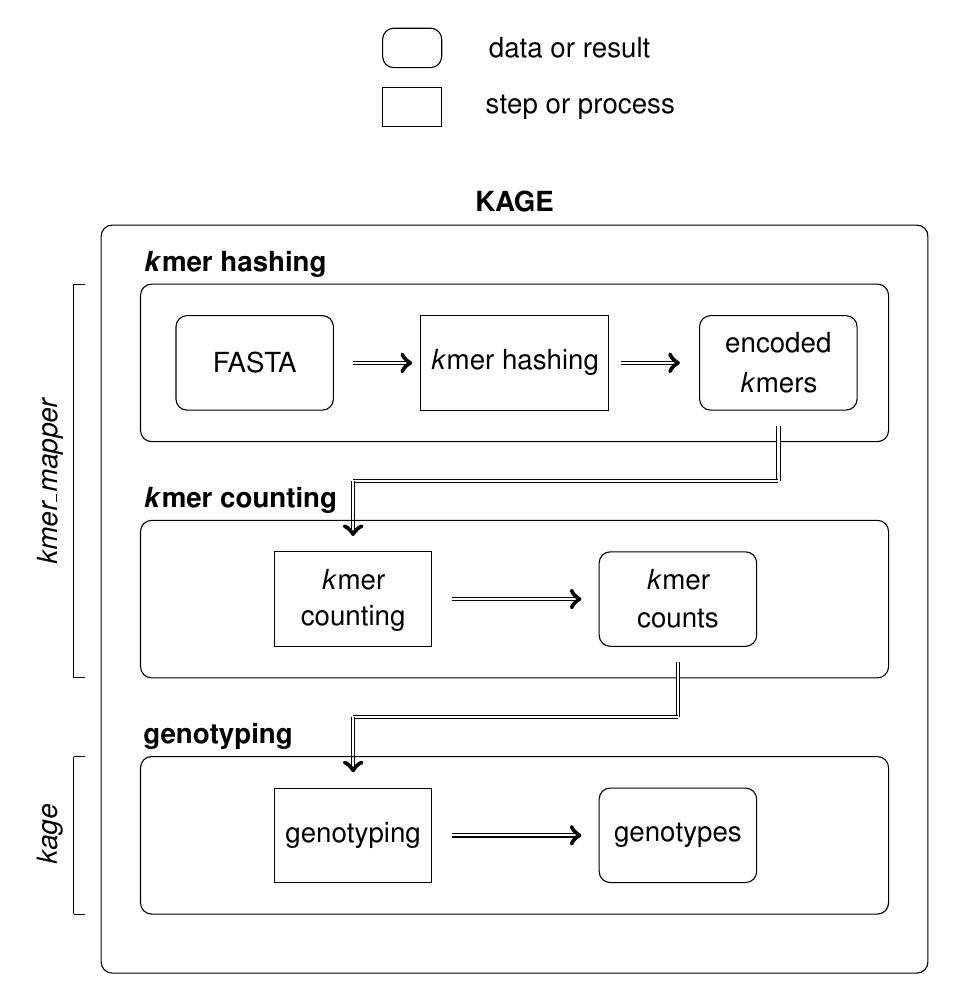
\begin{tikzpicture}
  % program hints
  % kmer_mapper
  \draw [](-2.3,1) -- (-2.3,-4);
  \draw [](-2.3,1) -- (-2.15,1);
  \draw [](-2.3,-4) -- (-2.15,-4);
  \node at(-2.6,-1.5)[rotate=90]{\fontfamily{phv}\selectfont\textit{\smaller{kmer\_mapper}}};
  % kage
  \draw [](-2.3,-5) -- (-2.3,-7);
  \draw [](-2.3,-5) -- (-2.15,-5);
  \draw [](-2.3,-7) -- (-2.15,-7);
  \node at(-2.6,-6)[rotate=90]{\fontfamily{phv}\selectfont\textit{\smaller{kage}}};
  % kmer hashing 
  \node at(-.25,1.25)[minimum width=2cm,minimum height=1.2cm](){\fontfamily{phv}\selectfont\smaller\textbf{\textit{k}mer hashing}};
  \node at(0,0)[draw,minimum width=2cm,minimum height=1.2cm,rounded corners](){\fontfamily{phv}\selectfont\smaller{FASTA}};
  \draw [double distance=.85pt,->](1.25,0) -- (2,0);
  \node at(3.3,0)[draw,minimum width=2cm,minimum height=1.2cm](){\fontfamily{phv}\selectfont\smaller{\textit{k}mer hashing}};
  \draw [double distance=.85pt,->](4.65,0) -- (5.4,0);
  \node at(6.65,0)[draw,minimum width=2cm,minimum height=1.2cm,rounded corners]{};
  \node at(6.65,.25)[]{\fontfamily{phv}\selectfont\smaller{encoded}};
  \node at(6.65,-.25)[]{\fontfamily{phv}\selectfont\smaller{\textit{k}mers}};
  \node at(3.3,0)[draw,minimum width=9.5cm,minimum height=2cm,rounded corners](){};
  % arrows
  \draw [double distance=.85pt](6.65,-.8) -- (6.65,-1.5);
  \draw [double distance=.85pt](6.65,-1.5) -- (1.25,-1.5);
  \draw [double distance=.85pt,->](1.25,-1.5) -- (1.25,-2.2);
  % kmer counting 
  \node at(-.185,-1.75)[minimum width=2cm,minimum height=1.2cm](){\fontfamily{phv}\selectfont\smaller\textbf{\textit{k}mer counting}};
  \node at(3.3,-3)[draw,minimum width=9.5cm,minimum height=2cm,rounded corners](){};
  \node at(1.25,-3)[draw,minimum width=2cm,minimum height=1.2cm]{};
  \node at(1.25,-2.75)[]{\fontfamily{phv}\selectfont\smaller{\textit{k}mer}};
  \node at(1.25,-3.25)[]{\fontfamily{phv}\selectfont\smaller{counting}};
  \draw [double distance=.85pt,->](2.5,-3) -- (4.15,-3);
  \node at(5.375,-3)[draw,minimum width=2cm,minimum height=1.2cm,rounded corners]{};
  \node at(5.375,-2.75)[]{\fontfamily{phv}\selectfont\smaller{\textit{k}mer}};
  \node at(5.375,-3.25)[]{\fontfamily{phv}\selectfont\smaller{counts}};
  % arrows
  \draw [double distance=.85pt](5.375,-3.8) -- (5.375,-4.5);
  \draw [double distance=.85pt](5.375,-4.5) -- (1.25,-4.5);
  \draw [double distance=.85pt,->](1.25,-4.5) -- (1.25,-5.2);
  % genotyping
  \node at(-.465,-4.75)[minimum width=2cm,minimum height=1.2cm](){\fontfamily{phv}\selectfont\smaller\textbf{genotyping}};
  \node at(3.3,-6)[draw,minimum width=9.5cm,minimum height=2cm,rounded corners](){};
  \node at(1.25,-6)[draw,minimum width=2cm,minimum height=1.2cm](){\fontfamily{phv}\selectfont\smaller{genotyping}};
  \draw [double distance=.85pt,->](2.5,-6) -- (4.15,-6);
  \node at(5.375,-6)[draw,minimum width=2cm,minimum height=1.2cm,rounded corners](){\fontfamily{phv}\selectfont\smaller{genotypes}};
  % KAGE
  \node at(3.3,2.05)[minimum width=2cm,minimum height=1.2cm](){\fontfamily{phv}\selectfont\smaller\textbf{KAGE}};
  \node at(3.3,-3)[draw,minimum width=10.5cm,minimum height=9.5cm,rounded corners](){};
  % Hints 
  \node at(2,4)[draw,minimum width=.75cm,minimum height=.5cm,rounded corners](){};
  \node at(4,4)[](){\fontfamily{phv}\selectfont data or result};
  \node at(2,3.25)[draw,minimum width=.75cm,minimum height=.5cm](){};
  \node at(4.135,3.25)[](){\fontfamily{phv}\selectfont step or process};
\end{tikzpicture}
}
\caption{
  A simplified overview of the KAGE genotyping pipeline.
  Three important parts of the pipeline are shown as distinct processes in the illustration: 
  1) \textbf{\textit{k}mer hashing}, which refers to the process of 2-bit encoding input reads from the fasta file and extracting - \textit{hashing} - all valid \textit{k}mers from those reads, 
  2) \textbf{\textit{k}mer counting}, which refers to the process of \textit{partial k}mer counting - counting the observed frequencies of a predefined set of \textit{k}mers in the input reads, and 
  3) \textbf{genotyping}, which refers to the process of computing the final genotype-probabilities supported by the observed \textit{k}mer counts.
  The \textit{k}mer hashing and counting and the genotyping are implemented in two pieces of software respectively: \textit{kmer\_mapper} and \textit{kage}.
}
\label{background:kage:figures:pipeline}
\end{center}
\end{figure}

